\chapter{Технологический раздел}
В данной части рассматривается выбор средств реализации, описывается структура классов программы и приводится интерфейс программного обеспечения.

\section{Средства реализации}
В данной работе для реализации был выбран язык программирования C++~\cite{C++}.

В качестве среды разработки была выбрана Qt Creator~\cite{Qt}.

Выбор обсуловлен наличием проработанной стандартной библиотеки, включающей в себя классы для работы с векторами и матрицами, большим количеством инструментов для работы с пользовательским интерфейсом. Используемые инструменты обладают полной функциональностью для разработки, профилирования и отладки необходимой программы.

\section{Структура программы}
Разработанное программное программное обеспечение состоит из следующих классов. Математические классы:
\begin{itemize}
    \item[---] QPointF --- класс для работы с точкой в двухмрном пространстве;
    \item[---] QVector3D --- класс для работы с трехмерными векторами;
    \item[---] QMatrix4x4 --- класс для работы с матрицами 4x4,
\end{itemize}
Классы для работы с объектами сцены:
\begin{itemize}
    \item[---] AbstractModel --- абстрактный класс объекта сцены;
    \item[---] Point --- класс точки в трехмерном пространстве;
    \item[---] Model --- класс представляющий трехмерное тело;
    \item[---] AbstractLight --- абстрактный класс источника света;
    \item[---] DirectionalLight --- класс направленного источника света;
    \item[---] AmbientLight --- класс фонового освещения.
\end{itemize}

Классы для визуализации сцены:
\begin{itemize}
    \item[---] Scene --- класс сцены;
    \item[---] AbstractDrawVisitor --- абстрактный класс посетителя для отрисовки объектов сцены;
    \item[---] DrawVisitor --- класс для отрисовки объекта заданным цветом;
    \item[---] DrawMappedVisitor --- класс для отрисовки объекта с визуализацией фактуры объекта;
    \item[---] DrawTextureVisitor --- класс для отрисовки с визуализацией текстуры объекта;
    \item[---] ProjectStrategy --- абстрактный класс стратегии процеирования трехмерной точки на плоскость;
    \item[---] PerspectiveStrategy --- класс перспективной процекуии точки на плоскость.
\end{itemize}

Классы интерфейса:
\begin{itemize}
    \item[---] MainWindow --- основное окно программы;
    \item[---] ModelViewer --- окно для просмотра тела вращения;
    \item[---] CurveCanvas --- холст для ввода пользователем направляющей.
\end{itemize}
Вспомогательные классы:
\begin{itemize}
    \item[---] Curve --- класс представления направляющей, введенной пользователем;
    \item[---] Facade --- класс для унификации доступа к сцене.
\end{itemize}

На рисунке~\ref{fig:classes} представлена диаграмма разработанных классов:
\begin{figure}[H]
	\centering
	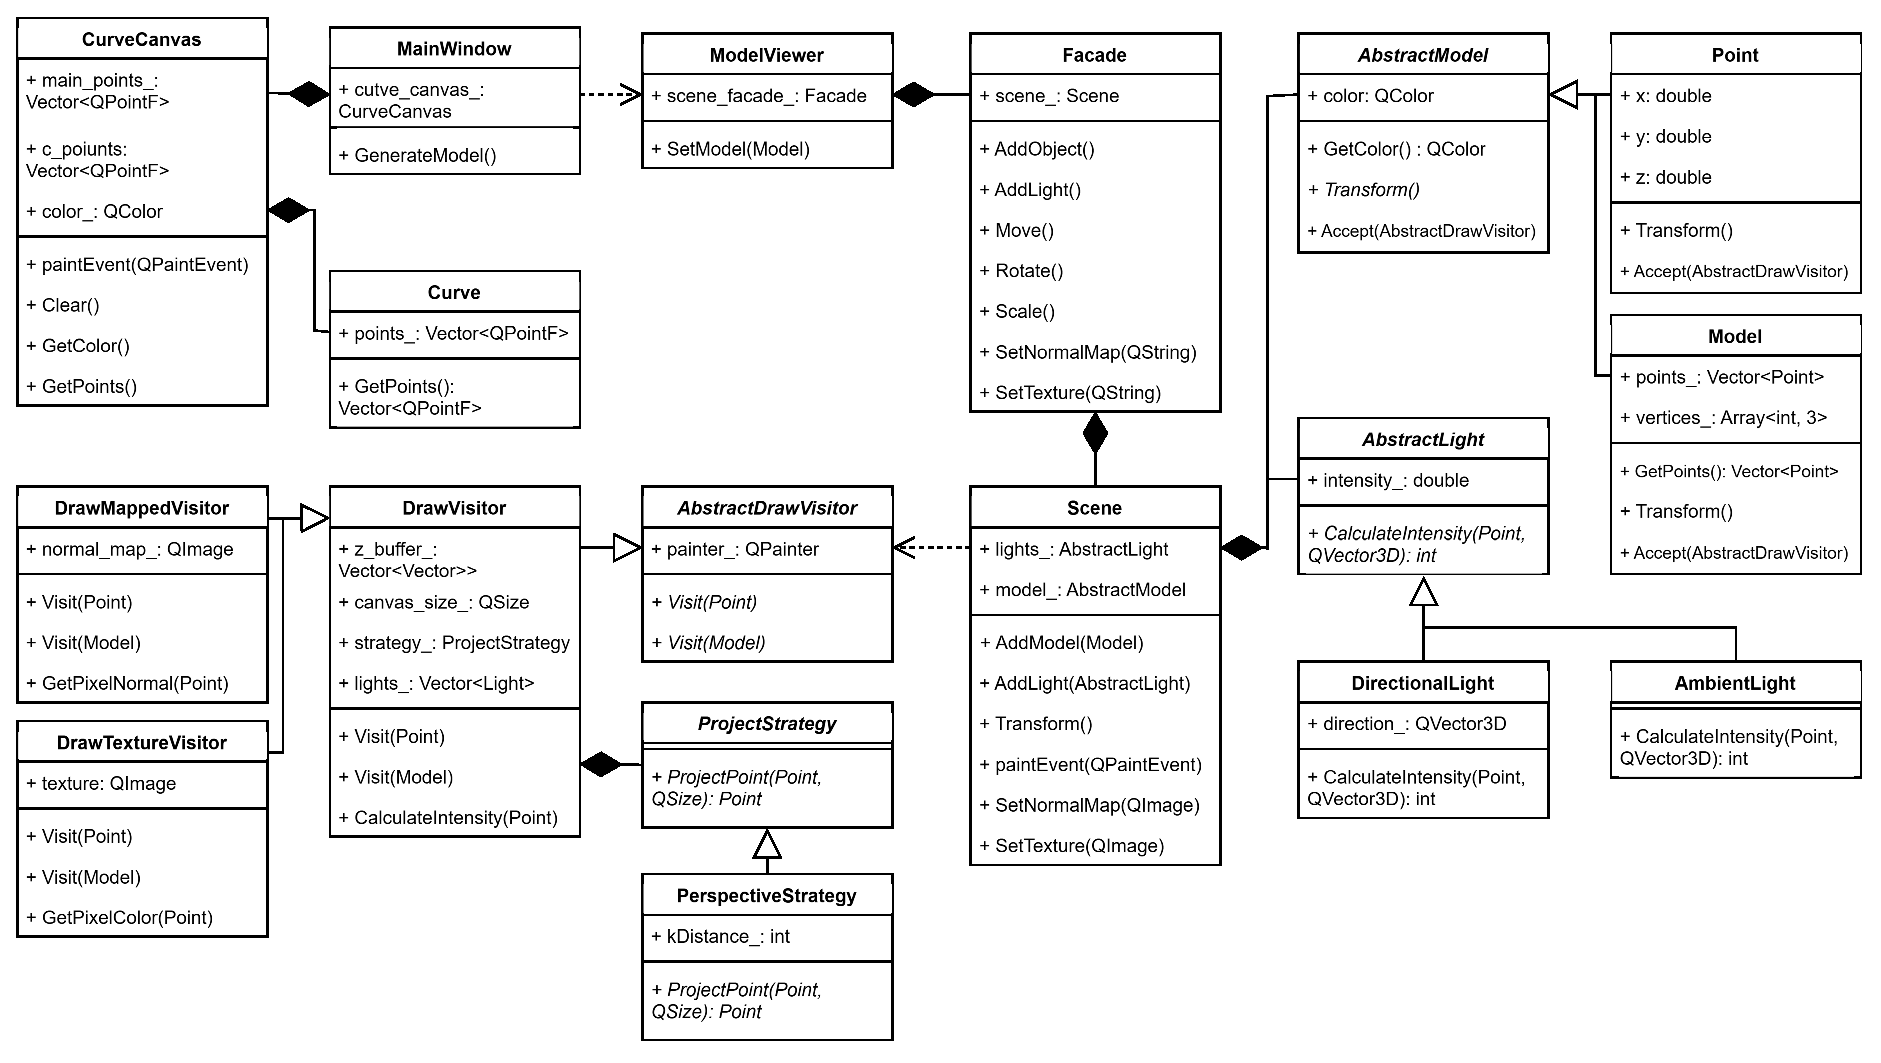
\includegraphics[scale=0.5]{img/classes.eps}
	\caption{Диаграмма классов программы}
	\label{fig:classes}
\end{figure}

\section{Схемы алгоритмов}
Схемы алгоритмов представлены на рисунках~\ref{fig:z_buffer}-~\ref{fig:rotate}
\begin{figure}[H]
	\centering
	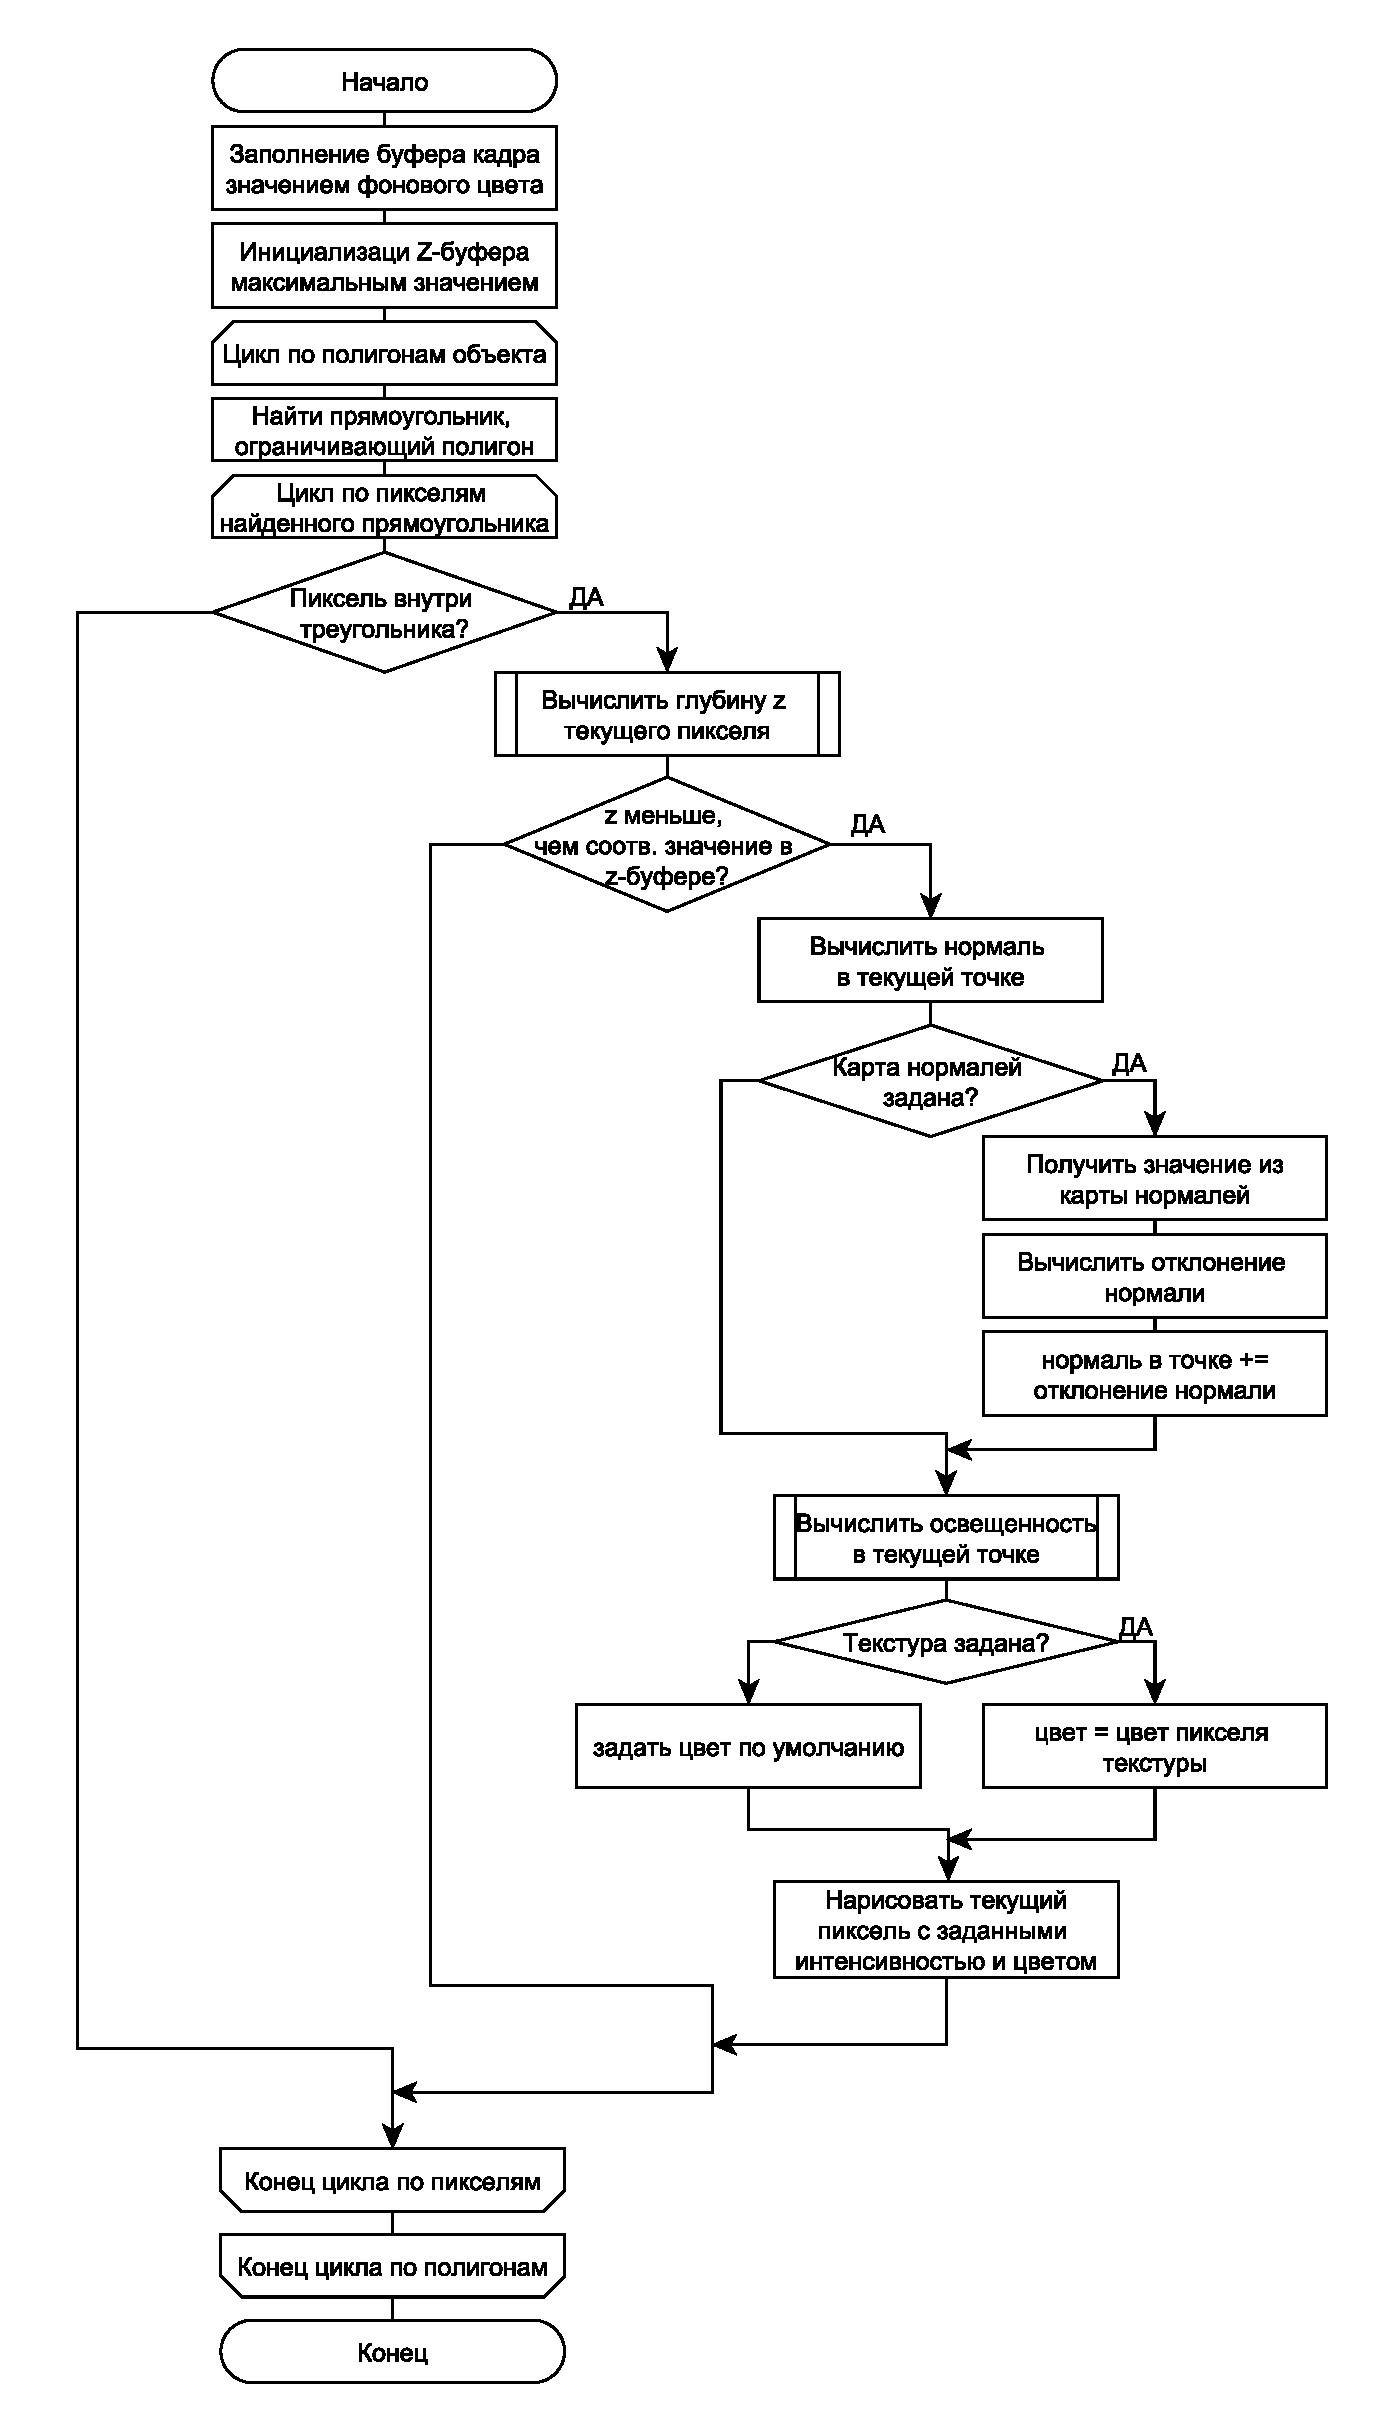
\includegraphics[scale=0.6]{img/Z_buf.eps}
	\caption{Схема алгоритма с Z-буфером}
	\label{fig:z_buffer}
\end{figure}

\begin{figure}[H]
	\centering
	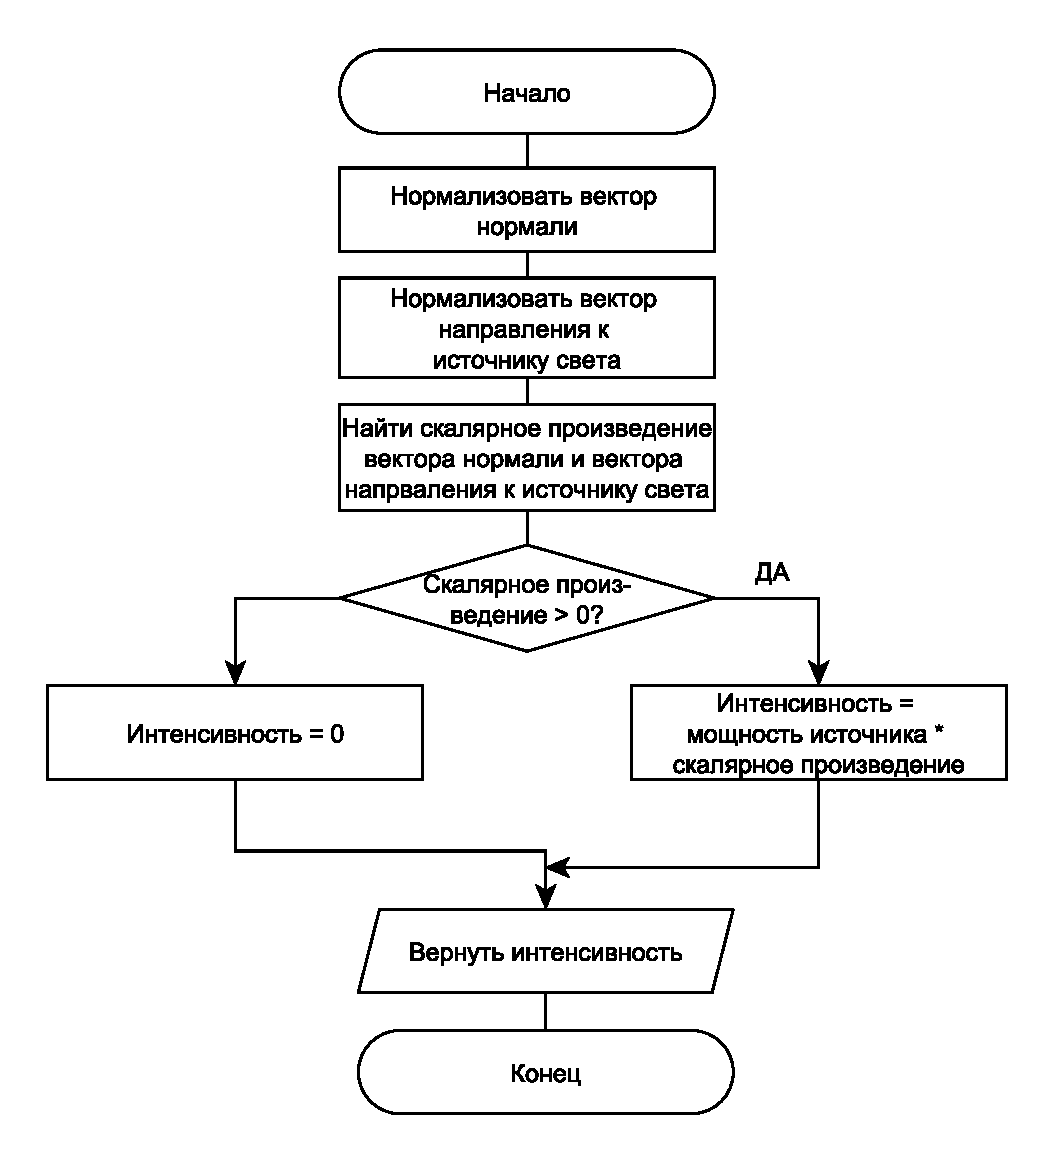
\includegraphics[scale=0.7]{img/light.eps}
	\caption{Схема алгоритма подсчета интенсивности света в точке}
	\label{fig:inten}
\end{figure}

\begin{figure}[H]
	\centering
	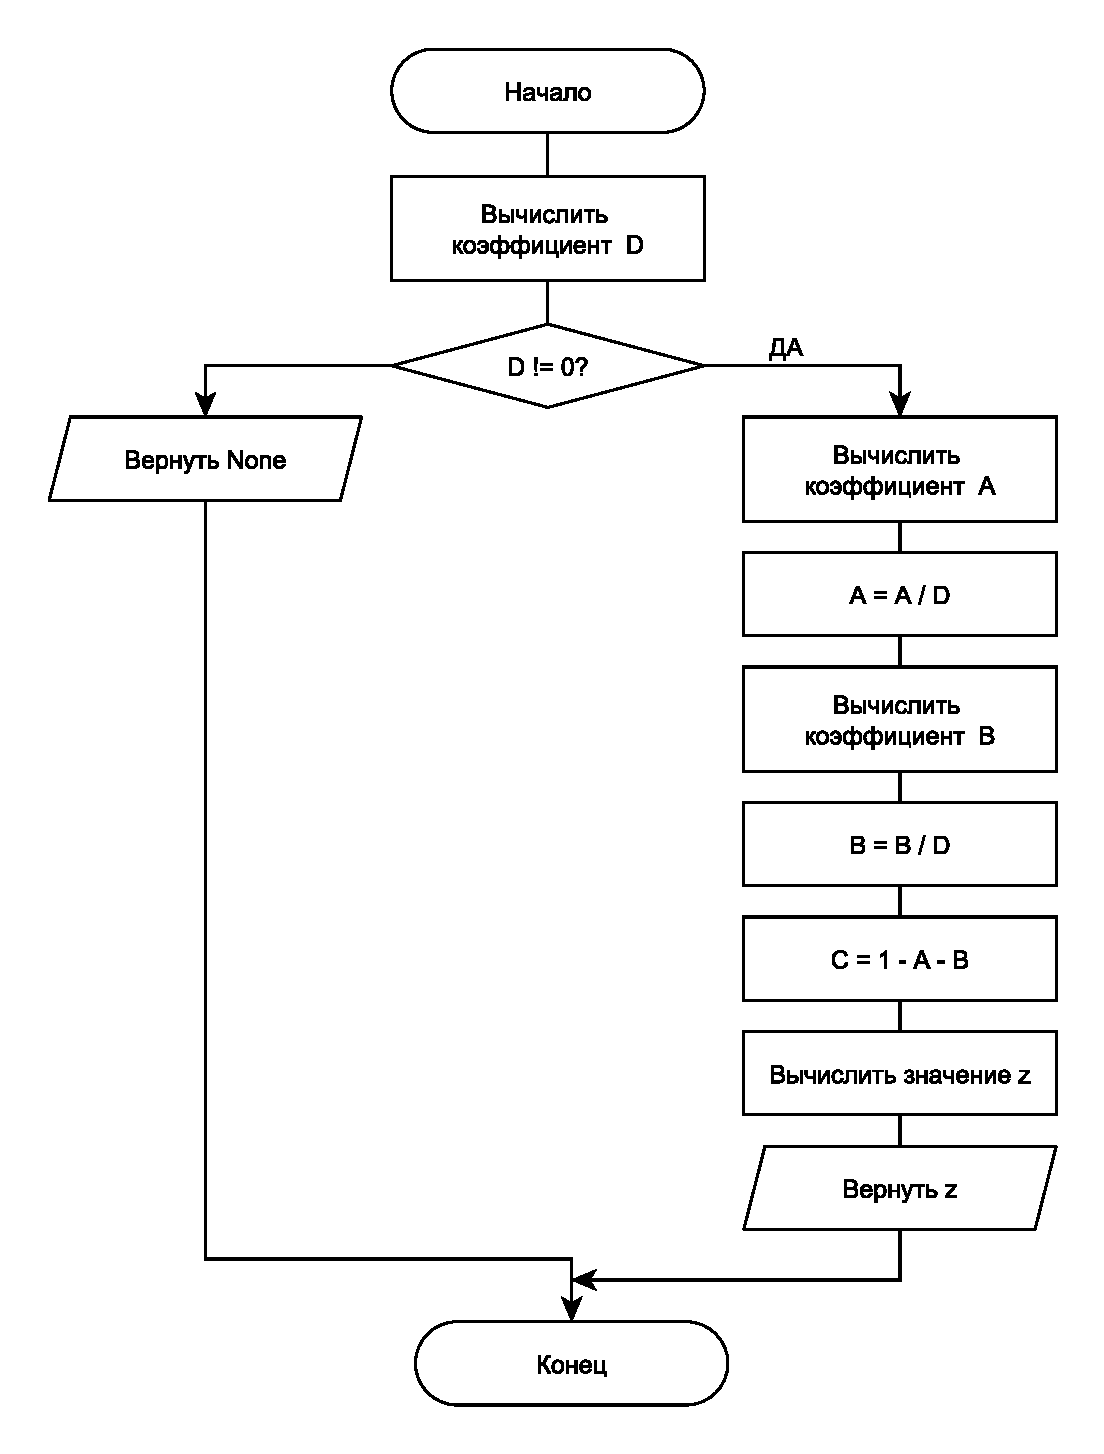
\includegraphics[scale=0.7]{img/bary.eps}
	\caption{Алгоритм вычисления значения глубины в точке}
	\label{fig:barry}
\end{figure}

\begin{figure}[H]
	\centering
	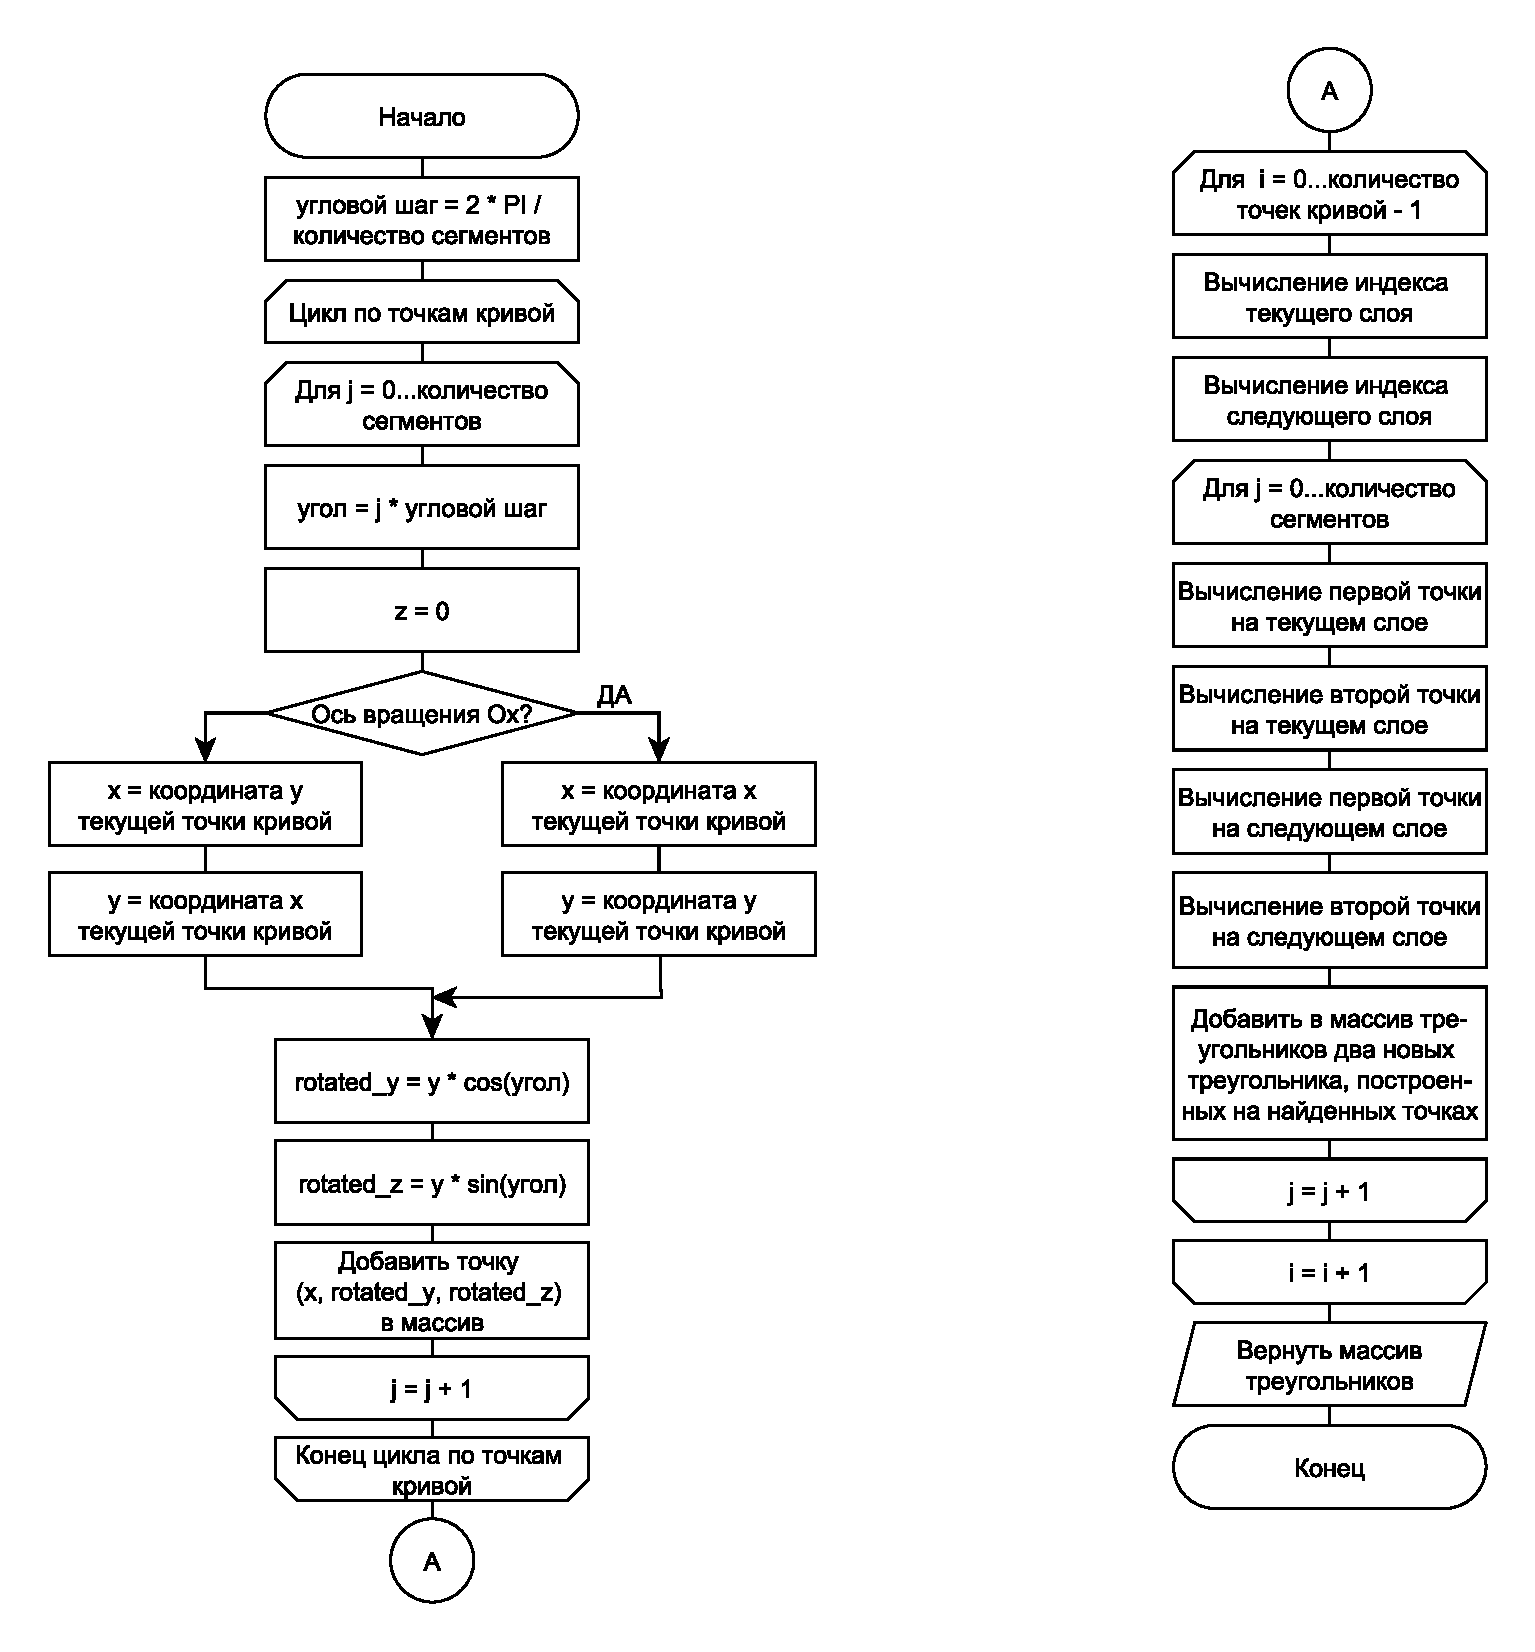
\includegraphics[scale=0.6]{img/rotate.eps}
	\caption{Алгоритм получения тела вращения}
	\label{fig:rotate}
\end{figure}

\section{Интерфейс программного обеспечения}
\begin{figure}[H]
	\centering
	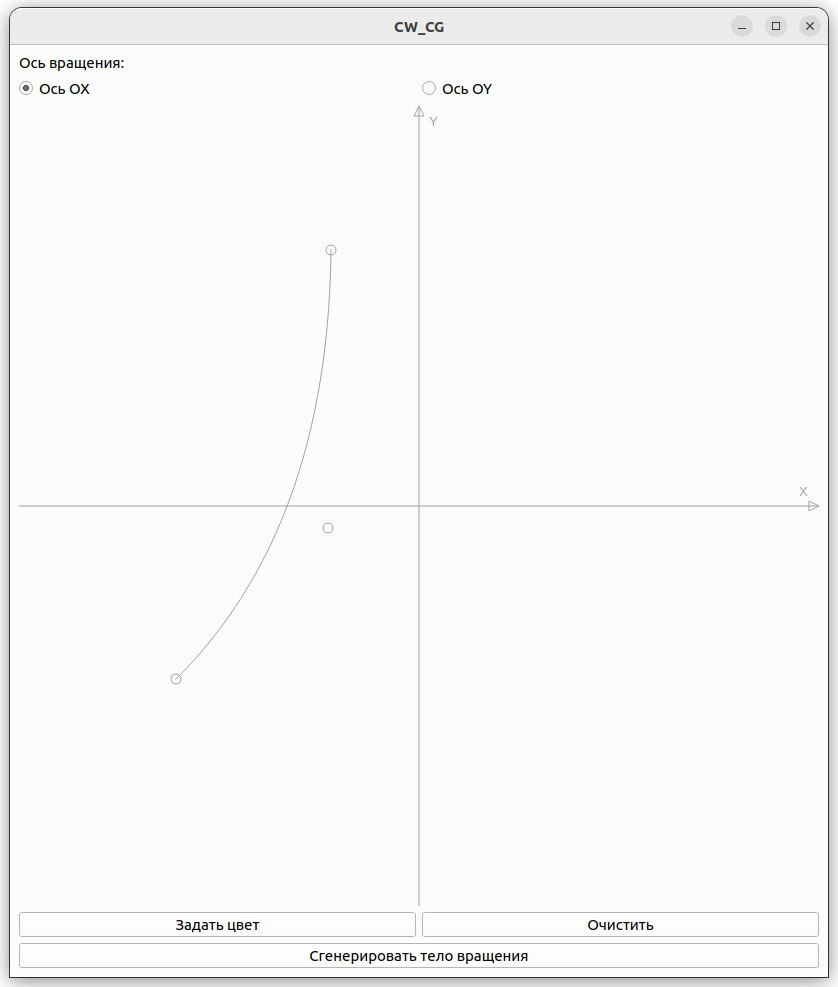
\includegraphics[scale=0.4]{img/inter_1.png}
	\caption{Графический интерфейс программы}
	\label{fig:main_window}
\end{figure}
Главное окно программы представлено на рисунке~\ref{fig:main_window}. При запуске программы в центре находится координатная плоскость для ввода пользователем направляющей. В верхней части окна находится список для выбора пользователем оси вращения. В нижней части окна находятся кнопки управления программой: кнопка задания цвета тела, кнопка очистки введенных точек, кнопки генерации тела вращения.

Пользователь вводит начальную и конечную точки нажатием левой кнопки мыши, а также необязательно задает контрольные точки правой кнопкой мыши, которые задают кривизну. При попытке ввести более двух начальных точек или ввести контрольные точки до задания начальных точек пользователь будет уведомлен ошибкой.

\begin{figure}[H]
	\centering
	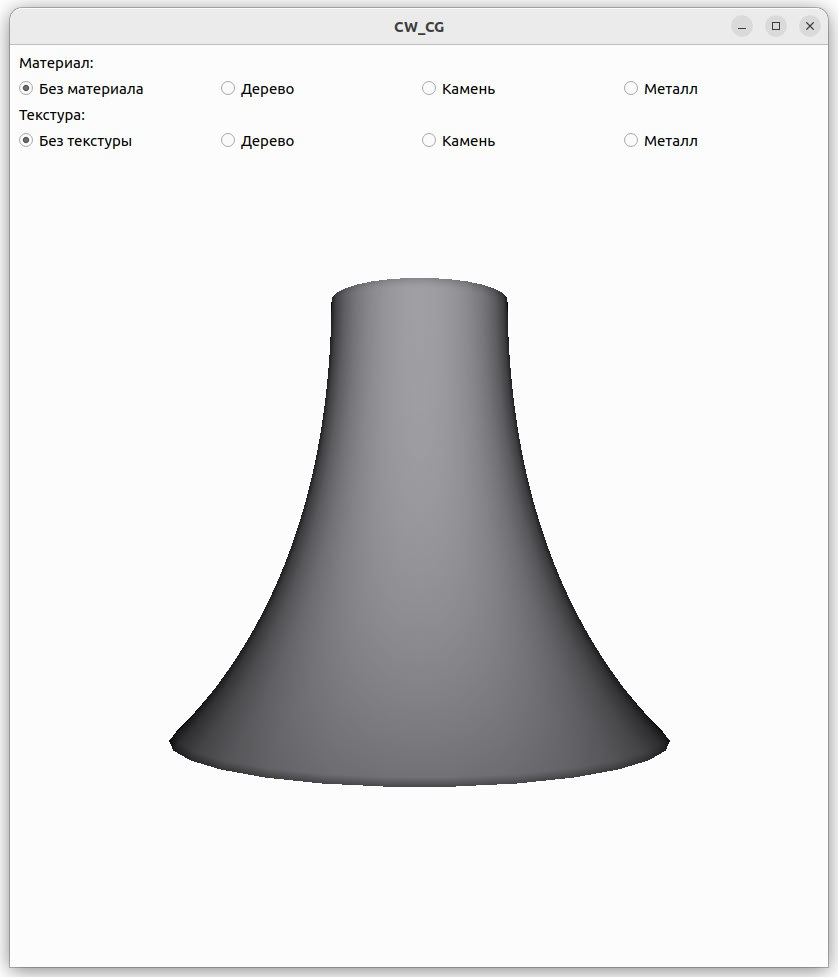
\includegraphics[scale=0.4]{img/inter_2.png}
	\caption{Окно просмотра полученного объекта}
	\label{fig:viewer}
\end{figure}
После генерации тела вращения оно актуализируется в новом окне. Окно визуализации представлено на рисунке~\ref{fig:viewer}. В верхней части экрана располагаются элементы управления визуализацией текстуры и фактуры материала.


\textbf{ВЫВОД}

В данном разделе были выбраны средства реализации, описаны структуры классов программы, описаны модули, а также рассмотрен интерфейс программы.

\clearpage